% !TeX program = xelatex
\documentclass[a4paper,10pt]{article}

% ============================================================================
% កញ្ចប់បណ្ណាល័យ (Packages) – តាមលំនាំ NGS Preah Krasang (ls_plan.tex)
% ============================================================================
\usepackage[a4paper, left=0.95cm, right=0.95cm, top=0.85cm, bottom=0.92cm, footskip=0.52cm]{geometry}
\usepackage{amsmath}
\usepackage{unicode-math}
\usepackage{fontspec}
\usepackage{array, longtable, multirow, colortbl}
\usepackage[table]{xcolor}
\usepackage{enumitem}
\usepackage{pifont}
\usepackage{fancyhdr}
\usepackage{tikz}
\usetikzlibrary{calc, arrows.meta, angles, quotes, decorations.markings, decorations.pathreplacing, patterns, babel}

% LaTeX 2025 + longtable v4.24 compatibility guard
\makeatletter
\let\@expl@@@mark@update@singlecol@structures@@\relax
\makeatother

% ============================================================================
% ការកំណត់ពុម្ពអក្សរ (Fonts Configuration - Cross-Platform Windows + Cloud fonts/)
% ============================================================================
\providecommand{\NGSFindFonts}{%
  \IfFileExists{C:/Windows/Fonts/cambria.ttc}{%
    \def\NGSSysPath{C:/Windows/Fonts/}%
    \def\NGSUserPath{C:/Users/KIT/AppData/Local/Microsoft/Windows/Fonts/}%
  }{%
    \IfFileExists{./fonts/KhmerOSsiemreap.ttf}{\def\NGSSysPath{./fonts/}\def\NGSUserPath{./fonts/}}{%
    \IfFileExists{../fonts/KhmerOSsiemreap.ttf}{\def\NGSSysPath{../fonts/}\def\NGSUserPath{../fonts/}}{%
    \IfFileExists{../../fonts/KhmerOSsiemreap.ttf}{\def\NGSSysPath{../../fonts/}\def\NGSUserPath{../../fonts/}}{%
    \IfFileExists{../../../fonts/KhmerOSsiemreap.ttf}{\def\NGSSysPath{../../../fonts/}\def\NGSUserPath{../../../fonts/}}{%
    \IfFileExists{../../../../fonts/KhmerOSsiemreap.ttf}{\def\NGSSysPath{../../../../fonts/}\def\NGSUserPath{../../../../fonts/}}{%
    \IfFileExists{../../../../../fonts/KhmerOSsiemreap.ttf}{\def\NGSSysPath{../../../../../fonts/}\def\NGSUserPath{../../../../../fonts/}}{%
    \IfFileExists{../../../../../../fonts/KhmerOSsiemreap.ttf}{\def\NGSSysPath{../../../../../../fonts/}\def\NGSUserPath{../../../../../../fonts/}}{%
      \def\NGSSysPath{../../../../../../../fonts/}\def\NGSUserPath{../../../../../../../fonts/}%
    }}}}}}}%
  }%
}
\NGSFindFonts

\setmathfont[
  Path={\NGSSysPath},
  FontIndex=1,
  Scale=1.02
]{cambria.ttc}

\defaultfontfeatures{Ligatures=TeX}

\setmainfont[
  Path={\NGSUserPath},
  Extension=.ttf,
  Script=Khmer,
  BoldFont={KhmerOSsiemreap},
  BoldFeatures={FakeBold=1.8},
  ItalicFont={KhmerOSsiemreap},
  ItalicFeatures={FakeSlant=0.25},
  BoldItalicFont={KhmerOSsiemreap},
  BoldItalicFeatures={FakeBold=1.8, FakeSlant=0.25}
]{KhmerOSsiemreap}

\newfontfamily\muol[
  Path={\NGSUserPath},
  Extension=.ttf,
  Script=Khmer
]{KhmerOSmuollight}

\newfontfamily\TimesEn[
  Path={\NGSSysPath},
  Extension=.ttf,
  Scale=1.00,
  BoldFont={timesbd},
  ItalicFont={timesi},
  BoldItalicFont={timesbi}
]{times}

\newfontfamily\NagaBold[
  Path={\NGSUserPath},
  Extension=.ttf
]{AKbalthom Naga Bold}

\newfontfamily\CalibriFont[
  Path={\NGSSysPath},
  Extension=.ttf
]{calibri}

\newfontfamily\Tacteing[
  Path={\NGSUserPath}
]{TACTENG.TTF}

\newfontfamily\CourierBullet[
  Path={\NGSSysPath},
  Extension=.ttf
]{cour}
\newcommand{\wcirc}{{\CourierBullet\fontsize{9.5pt}{11pt}\selectfont o}}

% ក្បួនកាត់ពាក្យខ្មែរ (Khmer word wrapping)
\XeTeXlinebreaklocale "km"
\XeTeXlinebreakskip = 0pt plus 1pt minus 0.1pt

% ============================================================================
% ការកំណត់ពណ៌ និងទម្រង់ទំព័រ (Colors & Page Style)
% ============================================================================
\definecolor{stepgray}{HTML}{D9D9D9}
\definecolor{headgray}{HTML}{F2F2F2}
\definecolor{boxgray}{HTML}{D9D9D9}
\definecolor{darkred}{HTML}{C00000}
\definecolor{red5e}{HTML}{FF0000}

\pagestyle{fancy}
\fancyhf{}
\renewcommand{\headrulewidth}{0pt}
\fancyfoot[R]{\CalibriFont\fontsize{11pt}{13pt}\selectfont\thepage}

\setlength{\parindent}{0pt}
\setlength{\parskip}{0pt}
\setlength{\tabcolsep}{3.8pt}

\newcolumntype{L}[1]{>{\raggedright\arraybackslash}p{#1}}

% ============================================================================
% ម៉ាក្រូជំនួយ (Helper Macros)
% ============================================================================
\newcommand{\en}[1]{{\TimesEn #1}}
\newcommand{\enbf}[1]{{\TimesEn\textbf{#1}}}
\newcommand{\unit}[1]{\,\text{\en{#1}}}
\newcommand{\fiveE}[1]{{\NagaBold\fontsize{9.5pt}{13pt}\selectfont\textcolor{red5e}{#1}}}
\newcommand{\timenote}[1]{\textcolor{darkred}{\textit{#1}}}
\newcommand{\redsub}[1]{\textcolor{darkred}{#1}}
\newcommand{\graybox}[1]{\colorbox{boxgray}{\strut\hspace{2pt}#1\hspace{2pt}}}
\newcommand{\ditem}{\tikz[baseline=-0.5ex]\fill (0,0.42ex) -- (0.42ex,0) -- (0,-0.42ex) -- (-0.42ex,0) -- cycle;\hspace{0.3em}}
\newcommand{\cnum}[1]{{\fontsize{10.5pt}{12pt}\selectfont\ding{\numexpr181+#1\relax}}\hspace{0.15em}}
\newcommand{\cfig}[1]{\par\vspace{4pt}{\centering #1\par}\vspace{4pt}}
\newcommand{\stepheader}[1]{\multicolumn{3}{|c|}{\cellcolor{stepgray}\muol #1} \\* \noalign{\hrule height 0.4pt}}
\newcommand{\fboxb}[1]{\begingroup\setlength{\fboxsep}{1.5pt}\fbox{#1}\endgroup}

% ក្បាច់ក្រោមបាវចនា (Tacteing Font - Keyboard '3')
\newcommand{\khmflourish}{{\Tacteing\fontsize{36pt}{14pt}\selectfont\raisebox{-5pt}{3}}}

% ============================================================================
% ម៉ាក្រូគូសរូប TikZ ស-ខ្មៅ ១០០% (Monochrome B&W TikZ Figures, Black Text, 4.5-7.4 cm)
% ============================================================================

% ១. ជំហានទី២ កំណែ ប្រតិបត្តិ 4.2 (ទំ.១៨ vs ទំ.១៧)
\newcommand{\figHWCheckPOWQ}{%
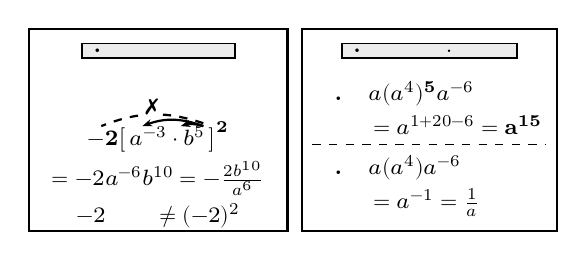
\begin{tikzpicture}[scale=0.90, every node/.style={font=\footnotesize, text=black}]
  % ឆ្វេង៖ សញ្ញាដកក្រៅវង់ក្រចក -2(a^{-3}b^5)^2
  \draw[black, line width=0.95pt] (0,0) rectangle (3.65,2.85);
  \node[fill=gray!15, draw=black, line width=0.6pt, inner sep=2pt] at (1.825,2.54) {\textbf{ក.} សញ្ញាដកក្រៅវង់ក្រចក};
  \node at (1.825,1.32) {$\mathbf{-2}\big[\,a^{-3}\cdot b^{5}\,\big]^{\mathbf{2}}$};
  \draw[black, line width=0.8pt, -{Stealth[length=3.5pt]}] (2.46,1.48) to[bend right=20] (1.60,1.48);
  \draw[black, line width=0.8pt, -{Stealth[length=3.5pt]}] (2.46,1.48) to[bend right=16] (2.14,1.48);
  \draw[black, line width=0.8pt, dashed] (2.46,1.52) to[bend right=20] node[above=-1pt, fill=white, inner sep=0.5pt]{\ding{55}} (1.02,1.48);
  \node at (1.825,0.74) {$= -2a^{-6}b^{10} = -\frac{2b^{10}}{a^6}$};
  \node at (1.825,0.22) {$-2$ នៅក្រៅ $\neq (-2)^2$};

  % ស្ដាំ៖ កំណត់សម្គាល់ពុម្ពទំ.១៧ vs ទំ.១៨
  \draw[black, line width=0.95pt] (3.85,0) rectangle (7.45,2.85);
  \node[fill=gray!15, draw=black, line width=0.6pt, inner sep=2pt] at (5.65,2.54) {\textbf{ខ.} ផ្ទៀងពុម្ពទំ.១៧ និង ១៨};
  \node[anchor=west] at (4.00,1.94) {\textbf{ទំ.១៧៖} $a(a^4)^{\mathbf{5}} a^{-6}$};
  \node[anchor=west] at (4.72,1.50) {$= a^{1+20-6} = \mathbf{a^{15}}$};
  \draw[black, line width=0.7pt, dashed] (4.00,1.22) -- (7.30,1.22);
  \node[anchor=west] at (4.00,0.90) {\textbf{ទំ.១៨៖} $a(a^4)a^{-6}$};
  \node[anchor=west] at (4.72,0.40) {$= a^{-1} = \frac{1}{a}$};
\end{tikzpicture}}

% ២. E1 Engage: បេសកកម្មធុងស្តុកទឹកគូប 1m -> (2/5)m
\newcommand{\figEngageTankPOWQ}{%
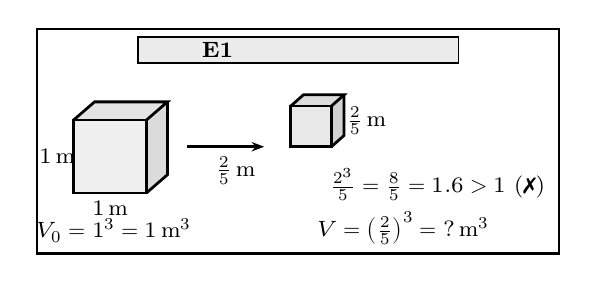
\begin{tikzpicture}[scale=0.89, every node/.style={font=\footnotesize, text=black}]
  \draw[black, line width=0.95pt] (0,0) rectangle (7.45,3.20);
  \node[fill=gray!15, draw=black, line width=0.6pt, inner sep=2pt] at (3.725,2.90) {\textbf{បេសកកម្ម \en{E1}៖ បង្រួមធុងស្តុកទឹកគូបនៅព្រះក្រសាំង}};

  % ធុងដើម 1m x 1m x 1m (បន្ថែមចន្លោះឆ្វេង-ស្ដាំស្អាត)
  \begin{scope}[shift={(0.52,0.86)}]
    \fill[gray!12] (0,0) rectangle (1.04,1.04);
    \fill[gray!22] (0,1.04) -- (0.30,1.30) -- (1.34,1.30) -- (1.04,1.04) -- cycle;
    \fill[gray!28] (1.04,0) -- (1.34,0.26) -- (1.34,1.30) -- (1.04,1.04) -- cycle;
    \draw[black, line width=1.0pt] (0,0) rectangle (1.04,1.04);
    \draw[black, line width=1.0pt] (0,1.04) -- (0.30,1.30) -- (1.34,1.30) -- (1.04,1.04);
    \draw[black, line width=1.0pt] (1.34,1.30) -- (1.34,0.26) -- (1.04,0);
    \node at (-0.23,0.52) {$1\unit{m}$};
    \node at (0.52,-0.22) {$1\unit{m}$};
    \node at (0.58,-0.54) {$V_0 = 1^3 = 1\unit{m}^3$};
  \end{scope}

  % ព្រួញបង្រួមគែម (ដាច់ច្បាស់ពីធុងដើម និងធុងតូច)
  \draw[black, line width=1.05pt, -{Stealth[length=4.5pt]}] (2.14,1.52) -- (3.24,1.52);
  \node at (2.69,1.86) {បង្រួមគែម};
  \node at (2.69,1.18) {មក $\frac{2}{5}\unit{m}$};

  % ធុងតូច (2/5)m
  \begin{scope}[shift={(3.62,1.52)}]
    \fill[gray!18] (0,0) rectangle (0.58,0.58);
    \fill[gray!28] (0,0.58) -- (0.18,0.74) -- (0.76,0.74) -- (0.58,0.58) -- cycle;
    \fill[gray!35] (0.58,0) -- (0.76,0.16) -- (0.76,0.74) -- (0.58,0.58) -- cycle;
    \draw[black, line width=1.0pt] (0,0) rectangle (0.58,0.58);
    \draw[black, line width=1.0pt] (0,0.58) -- (0.18,0.74) -- (0.76,0.74) -- (0.58,0.58);
    \draw[black, line width=1.0pt] (0.76,0.74) -- (0.76,0.16) -- (0.58,0);
    \node at (1.08,0.37) {$\frac{2}{5}\unit{m}$};
  \end{scope}
  \node[anchor=west] at (3.22,0.98) {\textbf{អន្ទាក់៖} $\frac{2^3}{5}=\frac{8}{5}=1.6>1$ (\ding{55})};
  \node[anchor=west] at (3.22,0.36) {\textbf{សំណួរ៖} $V = \left(\frac{2}{5}\right)^3 = ?\unit{m}^3$};
\end{tikzpicture}}

% ៣. E2 Act 1: ក្រឡាផ្ទៃឯកតា 5x5 និងបន្ទះកាត់ 2x2 + ផ្គុំកត្តា 2^3/5^3
\newcommand{\figExploreGridPOWQ}{%
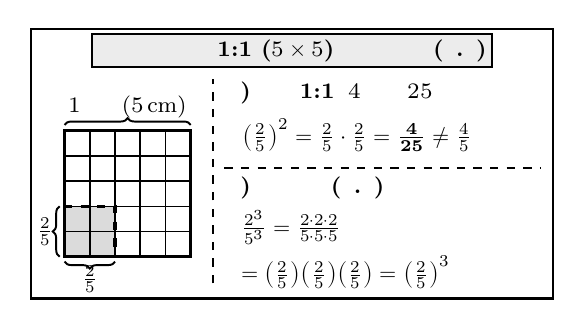
\begin{tikzpicture}[scale=0.89, every node/.style={font=\footnotesize, text=black}]
  \draw[black, line width=0.95pt] (0,0) rectangle (7.45,3.85);
  \node[fill=gray!15, draw=black, line width=0.6pt, inner sep=2pt] at (3.725,3.54) {\textbf{សកម្មភាព ១៖ ក្រឡា \en{1:1} ($5\times 5$) និងផ្គុំកត្តា (ទំ.១៨)}};

  % ក្រឡា 5x5 ជាមួយកែង 2x2 ឈូសប្រផេះ
  \begin{scope}[shift={(0.48,0.60)}]
    \fill[gray!28] (0,0) rectangle (0.72,0.72);
    \draw[black, line width=0.55pt] (0,0) grid[step=0.36] (1.80,1.80);
    \draw[black, line width=1.15pt] (0,0) rectangle (1.80,1.80);
    \draw[black, line width=1.15pt, dashed] (0,0) rectangle (0.72,0.72);
    % ប្រដាប់វាស់ 2/5 និង 1
    \draw[black, line width=0.7pt, decorate, decoration={brace, amplitude=2.5pt}] (0,1.88) -- (1.80,1.88);
    \node at (0.90,2.14) {$1$ ឯកតា ($5\unit{cm}$)};
    \draw[black, line width=0.7pt, decorate, decoration={brace, mirror, amplitude=2.5pt}] (0,-0.07) -- (0.72,-0.07);
    \node at (0.36,-0.32) {$\frac{2}{5}$};
    \draw[black, line width=0.7pt, decorate, decoration={brace, amplitude=2.5pt}] (-0.07,0) -- (-0.07,0.72);
    \node at (-0.28,0.36) {$\frac{2}{5}$};
  \end{scope}

  % ផ្នែកស្ដាំ៖ កំណត់សម្គាល់ផ្ទៀងផ្ទាត់ និងផ្គុំកត្តា
  \draw[black, line width=0.8pt, dashed] (2.60,0.22) -- (2.60,3.14);
  \node[anchor=west] at (2.76,2.94) {\textbf{១) ក្រឡា \en{1:1}៖} $4$ ក្នុង $25$ ការ៉េ};
  \node[anchor=west] at (2.88,2.34) {$\left(\frac{2}{5}\right)^2 = \frac{2}{5}\cdot\frac{2}{5} = \mathbf{\frac{4}{25}} \neq \frac{4}{5}$};
  \draw[black, line width=0.7pt, dashed] (2.76,1.86) -- (7.28,1.86);
  \node[anchor=west] at (2.76,1.58) {\textbf{២) ផ្គុំកត្តា (ទំ.១៨)៖}};
  \node[anchor=west] at (2.86,1.02) {$\frac{2^3}{5^3} = \frac{2\cdot 2\cdot 2}{5\cdot 5\cdot 5}$};
  \node[anchor=west] at (2.86,0.38) {$= \left(\frac{2}{5}\right)\!\left(\frac{2}{5}\right)\!\left(\frac{2}{5}\right) = \left(\frac{2}{5}\right)^3$};
\end{tikzpicture}}

% ៤. E2 Act 2A: POE 2A ក្រឡា 4x4 ជាមួយការ៉េឈូស 3x3
\newcommand{\figPOETwoAPOWQ}{%
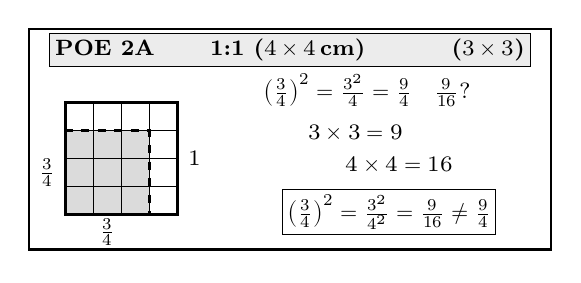
\begin{tikzpicture}[scale=0.89, every node/.style={font=\footnotesize, text=black}]
  \draw[black, line width=0.95pt] (0,0) rectangle (7.45,3.15);
  \node[fill=gray!15, draw=black, line width=0.6pt, inner sep=2pt] at (3.725,2.85) {\textbf{\en{POE 2A}៖ ក្រឡា \en{1:1} ($4\times 4\unit{cm}$) និងការ៉េឈូស ($3\times 3$)}};

  \begin{scope}[shift={(0.52,0.50)}]
    \fill[gray!28] (0,0) rectangle (1.20,1.20);
    \draw[black, line width=0.55pt] (0,0) grid[step=0.40] (1.60,1.60);
    \draw[black, line width=1.15pt] (0,0) rectangle (1.60,1.60);
    \draw[black, line width=1.1pt, dashed] (0,0) rectangle (1.20,1.20);
    \node at (-0.26,0.60) {$\frac{3}{4}$};
    \node at (0.60,-0.25) {$\frac{3}{4}$};
    \node at (1.84,0.80) {$1$};
  \end{scope}

  \node[anchor=west] at (2.74,2.28) {\textbf{ទាយ៖} $\left(\frac{3}{4}\right)^2 = \frac{3^2}{4} = \frac{9}{4}$ ឬ $\frac{9}{16}$?};
  \node[anchor=west] at (2.74,1.68) {\textbf{សង្កេត៖} ឈូស $3\times 3 = 9$ ការ៉េ};
  \node[anchor=west] at (3.12,1.22) {ក្នុងផ្ទៃសរុប $4\times 4 = 16$ ការ៉េ};
  \node[anchor=west] at (2.74,0.54) {\textbf{ពន្យល់៖} \fboxb{$\left(\frac{3}{4}\right)^2 = \frac{3^2}{4^2} = \frac{9}{16} \neq \frac{9}{4}$}};
\end{tikzpicture}}

% ៥. E2 Act 2B: POE 2B អន្ទាក់បំបែកលើផលបូក ((6+4)/2)^2 != (6^2+4^2)/2^2
\newcommand{\figPOETwoBPOWQ}{%
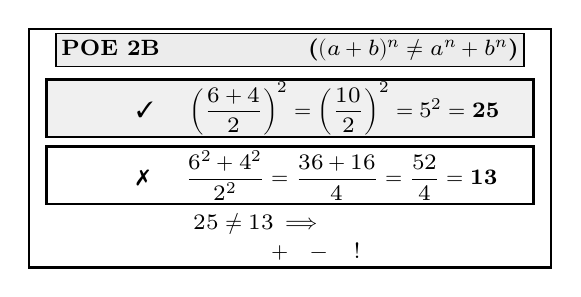
\begin{tikzpicture}[scale=0.89, every node/.style={font=\footnotesize, text=black}]
  \draw[black, line width=0.95pt] (0,0) rectangle (7.45,3.40);
  \node[fill=gray!15, draw=black, line width=0.6pt, inner sep=2pt] at (3.725,3.10) {\textbf{\en{POE 2B}៖ ឧទាហរណ៍ជំទាស់លើផលបូក ($(a+b)^n \neq a^n+b^n$)}};

  % ជួរលើ៖ ផ្លូវត្រូវ
  \draw[black, line width=1.0pt, fill=gray!12] (0.25,1.86) rectangle (7.20,2.68);
  \node[anchor=west] at (0.40,2.27) {\textbf{ផ្លូវត្រូវ} \ding{51}៖ \quad $\left(\dfrac{6+4}{2}\right)^2 = \left(\dfrac{10}{2}\right)^2 = 5^2 = \mathbf{25}$};

  % ជួរក្រោម៖ អន្ទាក់ខុស
  \draw[black, line width=0.95pt] (0.25,0.90) rectangle (7.20,1.72);
  \node[anchor=west] at (0.40,1.31) {\textbf{អន្ទាក់ខុស} \ding{55}៖ \quad $\dfrac{6^2+4^2}{2^2} = \dfrac{36+16}{4} = \dfrac{52}{4} = \mathbf{13}$};

  \node[align=center] at (3.725,0.44) {សង្កេត៖ $25 \neq 13 \implies$ ស្វ័យគុណ\textbf{មិនចែកចាយ}\\[1pt]លើសញ្ញា $+$ ឬ $-$ ឡើយ!};
\end{tikzpicture}}

% ៦. E3 Explain: ដ្យាក្រាម Hub-and-Spoke តភ្ជាប់លក្ខណៈទាំង ៣ ជុំវិញ x^n
\newcommand{\figExplainHubPOWQ}{%
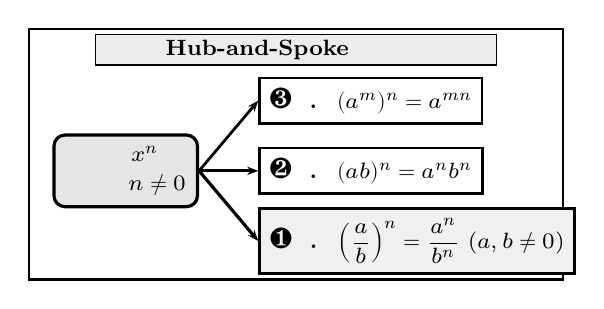
\begin{tikzpicture}[scale=0.91, every node/.style={font=\footnotesize, text=black}]
  \draw[black, line width=0.95pt] (0,0) rectangle (7.45,3.50);
  \node[fill=gray!15, draw=black, line width=0.6pt, inner sep=2pt] at (3.725,3.21) {\textbf{ដ្យាក្រាម \en{Hub-and-Spoke}៖ លក្ខណៈស្វ័យគុណទាំង ៣}};

  % មជ្ឈមណ្ឌល Hub
  \node[draw=black, line width=1.15pt, fill=gray!20, rounded corners=4pt, inner sep=4pt, align=center] (HUB) at (1.35,1.52) {\textbf{ស្នូល} $x^n$\\[1pt]និទស្សន្ត $n\neq 0$};

  % កាំទាំង ៣ Spokes
  \node[draw=black, line width=0.95pt, fill=white, inner sep=3.5pt, anchor=west] (S1) at (3.20,2.50) {\cnum{3} \textbf{៤.១៖} $(a^m)^n = a^{mn}$};
  \node[draw=black, line width=0.95pt, fill=white, inner sep=3.5pt, anchor=west] (S2) at (3.20,1.52) {\cnum{2} \textbf{៤.២៖} $(ab)^n = a^n b^n$};
  \node[draw=black, line width=1.15pt, fill=gray!12, inner sep=3.5pt, anchor=west] (S3) at (3.20,0.54) {\cnum{1} \textbf{៤.៣៖} $\left(\dfrac{a}{b}\right)^n = \dfrac{a^n}{b^n}$ ($a,b\neq 0$)};

  \draw[black, line width=1.0pt, -{Stealth[length=4pt]}] (HUB.east) -- (S1.west);
  \draw[black, line width=1.0pt, -{Stealth[length=4pt]}] (HUB.east) -- (S2.west);
  \draw[black, line width=1.15pt, -{Stealth[length=4pt]}] (HUB.east) -- (S3.west);
\end{tikzpicture}}

% ៧. E4 Elaborate: សញ្ញា [ចង្អុលអូស] ([tracing]) ពីនិទស្សន្តក្រៅទៅភាគយក និងភាគបែង
\newcommand{\figElaborateTracingPOWQ}{%
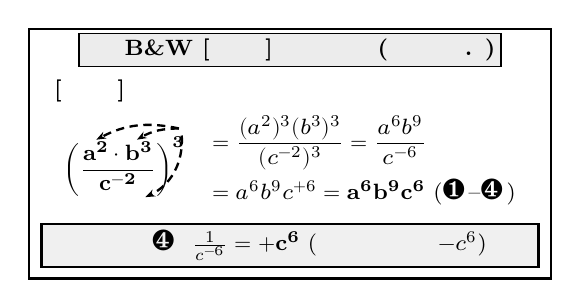
\begin{tikzpicture}[scale=0.89, every node/.style={font=\footnotesize, text=black}]
  \draw[black, line width=0.95pt] (0,0) rectangle (7.45,3.56);
  \node[fill=gray!15, draw=black, line width=0.6pt, inner sep=2pt] at (3.725,3.26) {\textbf{សញ្ញា \en{B\&W} [ចង្អុលអូស] ពីក្រៅចូលក្នុង (គំរូ ១ ខ ទំ.១៨)}};

  % កន្សោមដើម + ព្រួញអូស [tracing] (ដាច់ច្បាស់ពីស្លាក [ចង្អុលអូស])
  \node[anchor=west] at (0.22,2.68) {\textbf{[ចង្អុលអូស]}};
  \node at (1.36,1.60) {$\left(\dfrac{\mathbf{a^2}\cdot\mathbf{b^3}}{\mathbf{c^{-2}}}\right)^{\mathbf{3}}$};
  % ព្រួញអូសពីនិទស្សន្ត 3 ទៅលើ a^2, b^3, និង c^{-2} (កោងក្រោម y=2.38)
  \draw[black, line width=0.85pt, densely dashed, -{Stealth[length=3.5pt]}] (2.14,2.14) to[bend right=20] (0.96,1.98);
  \draw[black, line width=0.85pt, densely dashed, -{Stealth[length=3.5pt]}] (2.14,2.14) to[bend right=15] (1.54,1.98);
  \draw[black, line width=0.85pt, densely dashed, -{Stealth[length=3.5pt]}] (2.18,2.04) to[bend left=34] (1.66,1.16);

  % ជំហានបន្ត (២ បន្ទាត់ស្អាត)
  \node[anchor=west] at (2.48,1.94) {$= \dfrac{(a^2)^3 (b^3)^3}{(c^{-2})^3} = \dfrac{a^6 b^9}{c^{-6}}$};
  \node[anchor=west] at (2.48,1.24) {$= a^6 b^9 c^{+6} = \mathbf{a^6 b^9 c^6}$ (\cnum{1}--\cnum{4})};

  % ប្រអប់ប្រយ័ត្នច្រាស 1/c^{-6}
  \draw[black, line width=0.85pt, fill=gray!12] (0.18,0.16) rectangle (7.27,0.78);
  \node at (3.725,0.47) {\textbf{ប្រយ័ត្ន \cnum{4}៖} $\frac{1}{c^{-6}} = \mathbf{+c^6}$ (ត្រឡប់សញ្ញា មិនមែន $-c^6$)};
\end{tikzpicture}}

% ៨. E5 Exit Foils A–D (Printable ទំព័រ ៥)
\newcommand{\figExitCardsPOWQ}{%
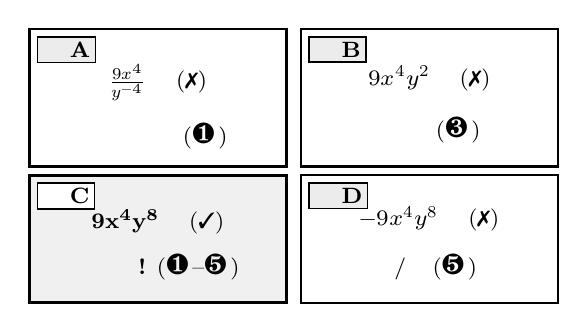
\begin{tikzpicture}[scale=0.92, every node/.style={font=\footnotesize, text=black}]
  % កាត A (X)
  \draw[black, line width=0.9pt] (0,1.72) rectangle (3.55,3.62);
  \node[anchor=north west, fill=gray!15, draw=black, line width=0.6pt, inner sep=1.8pt] at (0.10,3.52) {\textbf{កាត \en{A}}};
  \node at (1.775,2.88) {$\frac{9x^4}{y^{-4}}$ \quad (\ding{55})};
  \node at (1.775,2.14) {ភ្លេចលើកភាគបែង (\cnum{1})};

  % កាត B (X)
  \draw[black, line width=0.9pt] (3.75,1.72) rectangle (7.30,3.62);
  \node[anchor=north west, fill=gray!15, draw=black, line width=0.6pt, inner sep=1.8pt] at (3.85,3.52) {\textbf{កាត \en{B}}};
  \node at (5.525,2.94) {$9x^4 y^2$ \quad (\ding{55})};
  \node[align=center] at (5.525,2.26) {បូកនិទស្សន្ត\\ជំនួសគុណ (\cnum{3})};

  % កាត C (CHECK)
  \draw[black, line width=1.15pt, fill=gray!12] (0,-0.16) rectangle (3.55,1.60);
  \node[anchor=north west, fill=white, draw=black, line width=0.6pt, inner sep=1.8pt] at (0.10,1.50) {\textbf{កាត \en{C}}};
  \node at (1.775,0.96) {$\mathbf{9x^4 y^8}$ \quad (\ding{51})};
  \node at (1.775,0.34) {\textbf{ត្រឹមត្រូវ!} (\cnum{1}--\cnum{5})};

  % កាត D (X)
  \draw[black, line width=0.9pt] (3.75,-0.16) rectangle (7.30,1.60);
  \node[anchor=north west, fill=gray!15, draw=black, line width=0.6pt, inner sep=1.8pt] at (3.85,1.50) {\textbf{កាត \en{D}}};
  \node at (5.525,1.00) {$-9x^4 y^8$ \quad (\ding{55})};
  \node[align=center] at (5.525,0.38) {ខុសសញ្ញាដក\\គូ/សេស (\cnum{5})};
\end{tikzpicture}}

% ============================================================================
% ចាប់ផ្ដើមឯកសារ (Document Body — ចំនួនទំព័រ 4–8+ តាមខ្លឹមសារជាក់ស្ដែង, ពេញទំព័រ >=90%)
% ============================================================================
\begin{document}
\fontsize{10pt}{15.2pt}\selectfont

% -------------------- ក្បាលកិច្ចតែងការ (Header) --------------------
\begin{center}
  {\muol\fontsize{11pt}{16pt}\selectfont ព្រះរាជាណាចក្រកម្ពុជា}\\[2pt]
  {\muol\fontsize{10pt}{15pt}\selectfont ជាតិ សាសនា ព្រះមហាក្សត្រ}\\[1pt]
  \khmflourish
\end{center}

\vspace{-24pt}
{\muol\fontsize{9.5pt}{12.5pt}\selectfont
មន្ទីរអប់រំ យុវជន និងកីឡា ខេត្តកំពង់ធំ\\
ការិយាល័យអប់រំ យុវជន និងកីឡា ស្រុកកំពង់ស្វាយ\\
អនុវិទ្យាល័យព្រះក្រសាំង}

\vspace{1pt}
\begin{center}
  {\muol\fontsize{10pt}{14pt}\selectfont កិច្ចតែងការបង្រៀន}
\end{center}
\vspace{0pt}

% -------------------- ព័ត៌មានទូទៅ (Metadata) --------------------
{\renewcommand{\arraystretch}{0.98}
\hspace*{3.1cm}%
\begin{tabular}{@{}l l L{11.0cm}@{}}
  - \hspace{0.35cm} មុខវិជ្ជា & : & គណិតវិទ្យា ថ្នាក់ទី៨ (ពីជគណិត) \\
  - \hspace{0.35cm} ចំណងជើងមេរៀន & : & មេរៀនទី២៖ ស្វ័យគុណ \\
  - \hspace{0.35cm} ចំណងជើងរង & : & ២.៤.៣. ស្វ័យគុណនៃផលចែក និងពង្រឹងលក្ខណៈទាំង ៣ (ទំ.១៨, ២៥–២៦) \\
  - \hspace{0.35cm} រយៈពេល & : & ១ ម៉ោងសិក្សា (៥០ នាទី) \\
  - \hspace{0.35cm} បង្រៀនដោយ & : & ហុក ប៊ុនថែន \\
  - \hspace{0.35cm} កាលបរិច្ឆេទ & : & ថ្ងៃចន្ទ ទី១៦ ខែវិច្ឆិកា ឆ្នាំ២០២៦ \\
\end{tabular}

\vspace{2pt}

% -------------------- I. វត្ថុបំណង --------------------
\textbf{I.} {\muol វត្ថុបំណង}\\[1pt]
\hspace*{0.55cm}%
\begin{tabular}{@{}l l L{14.2cm}@{}}
  \wcirc \hspace{0.25cm} វិជ្ជាសម្បទា & : & សិស្សបង្គុំនិងប្រាប់រូបមន្តស្វ័យគុណនៃផលចែក $\left(\frac{a}{b}\right)^n = \frac{a^n}{b^n}$ (៤.៣ ទំ.១៨), ទំនាក់ទំនងពីរទិស $\frac{a^n}{b^n} = \left(\frac{a}{b}\right)^n$, និងច្បាប់ច្រាស $\left(\frac{a}{b}\right)^{-n} = \left(\frac{b}{a}\right)^n$ ($a,b\neq 0,\; n\neq 0$) ព្រមទាំងបែងចែកលក្ខណៈទាំង ៣ ។ \\
  \wcirc \hspace{0.25cm} បំណិនសម្បទា & : & សិស្សអនុវត្តពិសោធន៍ក្រឡា \en{1:1} ($5\times 5\unit{cm}$, $4\times 4\unit{cm}$), \en{Dual POE (2A, 2B)}, ប្រើ \textbf{[ចង្អុលអូស]} (\en{[tracing]}) និង \cnum{1}--\cnum{5} ដោះស្រាយលំហាត់គំរូទី 1 (ក, ខ, គ), ប្រតិបត្តិ (ទំ.១៨) និងកិច្ចការផ្ទះ ទំ.១៨, ២៥–២៦ បានត្រឹមត្រូវ ។ \\
  \wcirc \hspace{0.25cm} ចរិយាសម្បទា & : & សហការក្នុងក្រុម ៣ នាក់តាមវិន័យ \en{Pause-Ask / Pause-Review} និងប្រុងប្រយ័ត្នចំពោះអន្ទាក់ភ្លេចភាគបែង ការបំបែកលើផលបូក $(a\pm b)^n \neq a^n\pm b^n$ និងសញ្ញាដកក្រៅវង់ក្រចក ។ \\
\end{tabular}

\vspace{2pt}

% -------------------- II. សម្ភារៈឧបទេស --------------------
\textbf{II.} {\muol សម្ភារៈឧបទេស}\\[1pt]
\hspace*{0.55cm}$\bullet$ \hspace{0.35cm} សៀវភៅគោលទី៨ (ទំ.១៧–១៨, ២៥–២៦) បន្ទាត់ក្រិត \en{1:1} កន្ត្រៃ ខ្មៅដៃគូស \textbf{[ចង្អុលអូស]} កញ្ចប់ \en{1:1} (ទំព័រ ១) កាត \en{E4} (ទំព័រ ២) សន្លឹក \en{Relay E5} (ទំព័រ ៣) ផ្ទាំង \en{Hub-and-Spoke} \& \cnum{1}--\cnum{5} (ទំព័រ ៤) កាត \en{A--D} \& \en{Exit Ticket} (ទំព័រ ៥) និងប័ណ្ណកិច្ចការផ្ទះ (ទំព័រ ៦)

\vspace{2pt}

% -------------------- III. វិធីសាស្រ្តបង្រៀន --------------------
\textbf{III.} {\muol វិធីសាស្រ្តបង្រៀន}\\[1pt]
\hspace*{0.45cm}%
\begin{tabular}{@{}l l L{14.85cm}@{}}
  $\bullet$ \hspace{0.25cm} គោលវិធី & : & សិស្សមជ្ឈមណ្ឌល \\
  $\bullet$ \hspace{0.25cm} យុទ្ធវិធីបង្រៀន & : & ស្ថាបនានិយម គំរូ \en{5Es} (ក្រឡា \en{1:1}, \en{Dual POE}, \en{Hub-and-Spoke}, \textbf{[ចង្អុលអូស]}, \en{Relay} ៣ តួនាទី, លំហាត់ចម្រុះ) \\
\end{tabular}
}

\vspace{2pt}

% -------------------- IV. ដំណើរការបង្រៀន --------------------
\textbf{IV.} {\muol ដំណើរការបង្រៀន}

\vspace{1pt}

% ============================================================================
% តារាងដំណើរការបង្រៀន (Granular 2-5 Line Sub-Rows, Dedicated TikZ Rows, 50 min)
% ============================================================================
\renewcommand{\arraystretch}{1.15}
\begin{longtable}{|L{5.50cm}|L{7.90cm}|L{4.80cm}|}
\hline
\rowcolor{headgray}
\multicolumn{1}{|c|}{\muol សកម្មភាពគ្រូ} &
\multicolumn{1}{c|}{\muol ខ្លឹមសារមេរៀន} &
\multicolumn{1}{c|}{\muol សកម្មភាពសិស្ស} \\
\hline
\endfirsthead

\hline
\endhead

\hline
\endfoot

\hline
\endlastfoot

% ==================== ជំហានទី១ (2min) ====================
\stepheader{ជំហានទី១ \enbf{(}រដ្ឋបាលថ្នាក់\enbf{)}}
$\bullet$ ពិនិត្យអវត្តមាន អនាម័យ និងសណ្ដាប់ធ្នាប់ថ្នាក់រៀន
&
$\bullet$ រដ្ឋបាលថ្នាក់ \par
$\bullet$ អនាម័យ និងសុវត្ថិភាពកន្ត្រៃ/បន្ទាត់
&
$\circ$ ប្រធានថ្នាក់រាយការណ៍អវត្តមាន \\[3pt]

$\bullet$ រៀបចំសិស្សជាក្រុម ៣ នាក់ («ក្រុមអ្នកស៊ើបអង្កេតស្វ័យគុណ ៣ តួនាទី») \par
$\bullet$ ចែកកញ្ចប់ \en{1:1} (\en{Printable} ទំព័រ ១) ផ្កាប់លើតុ
&
$\bullet$ ត្រៀមក្រុម ៣ នាក់ និងរៀបចំសម្ភារៈ \en{B\&W} (កន្ត្រៃ បន្ទាត់ \en{1:1} ខ្មៅដៃ)
&
$\circ$ អង្គុយតាមក្រុម ៣ នាក់ និងដាក់សន្លឹក ១:១ ផ្កាប់លើតុ \\
\hline

% ==================== ជំហានទី២ (9min: <=3 + 3 + E1 3) ====================
\stepheader{ជំហានទី២ \enbf{(}កិច្ចការផ្ទះ \enbf{+} ទំនាក់ទំនងមេរៀនថ្មី\enbf{)}}
% --- ២.១ កំណែកិច្ចការផ្ទះ (<=3min) ---
\ditem \textbf{កំណែកិច្ចការផ្ទះ ($\le 3\unit{min}$)} \timenote{(កុំសរសេរវែង)} \par
$\bullet$ ហៅសិស្សឡើងផ្ទៀង \textbf{ប្រតិបត្តិ ៤.២ (ទំ.១៨)} ក. និង ខ. \par
\hspace*{0.3em}– \textbf{សំណួរ (ក)៖} «ហេតុអ្វី $-2$ មិនត្រូវលើកជា $(-2)^2 = +4$?»
&
{\centering\redsub{កំណែកិច្ចការផ្ទះមេរៀនមុន (ប្រតិបត្តិ ៤.២ ទំ.១៨)}\par} \par
$\bullet$ \textbf{ក.} $-2(a^{-3}\cdot b^5)^2 = -2(a^{-6}\cdot b^{10})$ \par
$\phantom{\bullet\ \textbf{ក.}} = -2a^{-6}b^{10} = -\dfrac{2b^{10}}{a^6}$ \quad ($a\neq 0$) \par
\timenote{(សង្កត់ធ្ងន់៖ $-2$ នៅក្រៅវង់ក្រចក មិនមែន $(-2)^2$ ទេ!)}
&
$\circ$ ផ្ទៀងលំហាត់ \textbf{ក.} និងឆ្លើយ៖ «$-2$ ស្ថិតនៅក្រៅវង់ក្រចក រក្សាសញ្ញាដក!» \\[3pt]

$\bullet$ ផ្ទៀង \textbf{ខ.} និងបញ្ជាក់ភាពខុសគ្នានៃពុម្ពសៀវភៅទំ.១៧ vs ទំ.១៨
&
$\bullet$ \textbf{ខ.} $a\cdot(a^4)^5\cdot a^{-6} = a^1\cdot a^{20}\cdot a^{-6} = a^{15}$ \quad ($a\neq 0$) \par
\textit{(កំណត់សម្គាល់ពុម្ពទំ.១៨៖ បាត់និទស្សន្ត $5$ ក្រៅ $(a^4)$ ក្លាយជា $a\cdot(a^4)\cdot a^{-6} = a^{1+4-6} = a^{-1} = \frac{1}{a}$)}
&
$\circ$ ផ្ទៀងចម្លើយ $a^{15}$ និងកត់សម្គាល់ពុម្ពទំ.១៨ ($a^{-1}$) \\[3pt]

&
\cfig{\figHWCheckPOWQ}
& \\[3pt]

% --- ២.២ រំលឹកមេរៀនចាស់ (3min) ---
\ditem \textbf{រំលឹកមេរៀនទាក់ទង (3min)} \par
$\bullet$ សួររំលឹកច្បាប់វិធីចែក (§3), ស្វ័យគុណនៃស្វ័យគុណ (§4.1), និងស្វ័យគុណនៃផលគុណ (§4.2) \par
\hspace*{0.3em}– \textbf{សំណួរ៖} «តើ $\frac{a^m}{a^n}$, $(a^m)^n$, និង $(ab)^n$ ស្មើអ្វី?»
&
{\centering\redsub{រំលឹកមេរៀនទាក់ទងមេរៀនថ្មី}\par} \par
$\bullet$ \textbf{§3 វិធីចែក៖} $\dfrac{a^m}{a^n} = a^{m-n},\; a^0 = 1,\; a^{-n} = \dfrac{1}{a^n}$ ($a\neq 0$) \par
$\bullet$ \textbf{§4.1៖} $(a^m)^n = a^{mn}$ \quad \textbar{} \quad \textbf{§4.2៖} $(ab)^n = a^n b^n$
&
$\circ$ ឆ្លើយរំលឹករូបមន្ត §3, §4.1, និង §4.2 ព្រមទាំងលក្ខខណ្ឌ $a\neq 0$ \\[3pt]

% --- ២.៣ E1 Engage (3min) ---
\fiveE{E1 - Engage (3min)} \timenote{(កុំទាន់ផ្ដល់ចម្លើយ)} \par
\ditem \textbf{«បេសកកម្មកាត់បង្រួមធុងស្តុកទឹក និងផ្ទាំងសំណាញ់នៅព្រះក្រសាំង»} \par
$\bullet$ ឱ្យសិស្សសង្កេតធុងគូប $1\unit{m}$ បង្រួមគែមមក $\frac{2}{5}\unit{m}$ និងអន្ទាក់ $\frac{2^3}{5} = \frac{8}{5}\unit{m}^3$
&
{\centering\redsub{បេសកកម្ម E1៖ ធុងស្តុកទឹកគូបនៅព្រះក្រសាំង}\par} \par
$\bullet$ ធុងដើមគែម $1\unit{m} \implies$ មាឌ $V_0 = 1^3 = 1\unit{m}^3$ \par
$\bullet$ កាត់បង្រួមគែមមក $\dfrac{2}{5}\unit{m} \implies$ មាឌថ្មី $V = \left(\dfrac{2}{5}\right)^3 = ?\unit{m}^3$
&
$\circ$ សង្កេតបញ្ហាធុងស្តុកទឹកគូប \\[3pt]

&
\cfig{\figEngageTankPOWQ}
& \\[3pt]

\hspace*{0.3em}– \textbf{សំណួរ៖} «សិស្សម្នាក់គណនា $\frac{2^3}{5} = \frac{8}{5} = 1.6\unit{m}^3$! តើធុងតូចជាងដើម អាចផ្ទុកទឹកច្រើនជាងធុង $1\unit{m}^3$ ដើមបានឬទេ? ហេតុអ្វី?»
&
$\bullet$ \textbf{អន្ទាក់ភ្លេចភាគបែង៖} $\dfrac{2^3}{5} = \dfrac{8}{5} = 1.6\unit{m}^3 > 1\unit{m}^3$ \par
$\bullet$ \textbf{ចម្ងល់៖} ហេតុអ្វីគម្លាតលទ្ធផលខុសឆ្ងាយម៉្លេះ? តើត្រូវលើកស្វ័យគុណត្រង់ណាខ្លះ?
&
$\circ$ ស្រង់ការទស្សន៍ទាយក្រុមទុកលើក្ដារខៀន (មិនទាន់បញ្ជាក់) \\
\hline

% ==================== ជំហានទី៣ (17min: E2 11m + E3 6m) ====================
\stepheader{ជំហានទី៣ \enbf{(}ខ្លឹមសារមេរៀនថ្មី\enbf{)}}
% --- ៣.១ ចំណងជើង & E2 Act 1 (5min) ---
\fiveE{E2 - Explore (11min)} \par
$\bullet$ សរសេរចំណងជើងមេរៀនលើក្ដារខៀន
&
មេរៀនទី២ \hspace{0.15cm} {\muol ស្វ័យគុណ} \textbf{(ត)} \par
\textbf{៤. លក្ខណៈនៃស្វ័យគុណ (ត)} \par
៤.៣. ស្វ័យគុណនៃផលចែក និងពង្រឹងលក្ខណៈទាំង ៣
&
$\circ$ កត់ចំណងជើងមេរៀនចូលសៀវភៅ \\[3pt]

\ditem \textbf{សកម្មភាព ១៖ ពិសោធន៍ក្រឡា \en{1:1} និងផ្គុំកត្តា (5min, ទំព័រ ១)} \par
$\bullet$ ផ្ទៀងបន្ទាត់ \en{calibration} $5.00\unit{cm}$ (\en{Actual Size 100\%}) \par
$\bullet$ កាត់បន្ទះឈូស $2.00\times 2.00\unit{cm}$ ដាក់លើក្រឡាឯកតា $5.00\times 5.00\unit{cm}$ ($25$ ការ៉េ)
&
{\centering\textbf{សកម្មភាព ១៖ ក្រឡាឯកតា $5\times 5\unit{cm}$ និងឧទាហរណ៍ (ទំ.១៨)}\par} \par
$\bullet$ \textbf{ក្រឡា \en{1:1}៖} បន្ទះ $\frac{2}{5}\times\frac{2}{5}$ គ្រប $4$ ការ៉េតូច ក្នុងចំណោម $25$ ការ៉េតូច \par
$\implies \left(\dfrac{2}{5}\right)^2 = \dfrac{4}{25} = \dfrac{2^2}{5^2} \neq \dfrac{4}{5}$
&
$\circ$ ផ្ទៀងបន្ទាត់ $5.00\unit{cm}$, កាត់បន្ទះ $2\times 2\unit{cm}$ ដាក់លើក្រឡា $5\times 5\unit{cm}$ និងរាប់ $4/25$ \\[3pt]

$\bullet$ ដឹកនាំផ្គុំកត្តាពី \textbf{ឧទាហរណ៍ (ទំ.១៨)} ក. \par
\hspace*{0.3em}– \textbf{សំណួរ៖} «ពេលមាននិទស្សន្តដូចគ្នាទាំងលើទាំងក្រោម តើផ្គុំជាស្វ័យគុណនៃផលចែកដូចម្ដេច?»
&
$\bullet$ \textbf{ឧទាហរណ៍ ក៖} $\dfrac{2^3}{5^3} = \dfrac{\overbrace{2\times 2\times 2}^{3\text{ កត្តា}}}{\underbrace{5\times 5\times 5}_{3\text{ កត្តា}}} = \underbrace{\left(\dfrac{2}{5}\right)\left(\dfrac{2}{5}\right)\left(\dfrac{2}{5}\right)}_{3\text{ កត្តា}} = \left(\dfrac{2}{5}\right)^3$
&
$\circ$ ផ្គុំគូកត្តា $\left(\frac{2}{5}\right)$ \\[3pt]

$\bullet$ ឱ្យសិស្សទាញរូបមន្តទូទៅពី \textbf{ឧទាហរណ៍ ខ.}
&
$\bullet$ \textbf{ឧទាហរណ៍ ខ៖} $\dfrac{a^n}{b^n} = \dfrac{\overbrace{a\cdot a\cdots a}^{n\text{ កត្តា}}}{\underbrace{b\cdot b\cdots b}_{n\text{ កត្តា}}} = \underbrace{\left(\dfrac{a}{b}\right)\cdots\left(\dfrac{a}{b}\right)}_{n\text{ កត្តា}} = \left(\dfrac{a}{b}\right)^n$
&
$\circ$ សង្ខេបរូបមន្ត $\left(\frac{a}{b}\right)^n$ \\[3pt]

&
\cfig{\figExploreGridPOWQ}
& \\[3pt]

% --- ៣.២ E2 Act 2 Dual POE (6min) ---
\ditem \textbf{សកម្មភាព ២៖ \en{Dual POE} (6min, ទំព័រ ១)} \par
$\bullet$ \textbf{\en{POE 2A} (\en{1:1} $4.00\times 4.00\unit{cm}$ ឈូស $3.00\times 3.00\unit{cm}$)៖} \par
\hspace*{0.3em}– ឱ្យសិស្ស \textbf{ទស្សន៍ទាយ} មុនរាប់ការ៉េឈូស ($9$ ក្នុង $16$) \par
\hspace*{0.3em}– \textbf{សំណួរ៖} «ហេតុអ្វី $\left(\frac{3}{4}\right)^2 \neq \frac{9}{4}$?»
&
{\centering\textbf{\en{POE 2A}៖ ទស្សន៍ទាយ -- សង្កេត -- ពន្យល់ ($\left(\frac{3}{4}\right)^2$)}\par} \par
$\bullet$ \textbf{ទាយ៖} សិស្សខ្លះស្មាន $\frac{3^2}{4} = \frac{9}{4} = 2.25 > 1$ \par
$\bullet$ \textbf{សង្កេត៖} ផ្នែកឈូសមាន $3\times 3 = 9$ ការ៉េ ក្នុងផ្ទៃសរុប $4\times 4 = 16$ ការ៉េ \par
$\bullet$ \textbf{ពន្យល់៖} \graybox{$\left(\dfrac{3}{4}\right)^2 = \dfrac{3^2}{4^2} = \dfrac{9}{16} \neq \dfrac{9}{4}$}
&
$\circ$ ទស្សន៍ទាយ រាប់ការ៉េ $9/16$ និងពន្យល់បដិសេធ $9/4$ \\[3pt]

&
\cfig{\figPOETwoAPOWQ}
& \\[3pt]

$\bullet$ \textbf{\en{POE 2B} (ឧទាហរណ៍ជំទាស់លើផលបូក)៖} \par
\hspace*{0.3em}– ឱ្យសិស្សទស្សន៍ទាយតម្លៃ $\left(\frac{6+4}{2}\right)^2$ ធៀប $\frac{6^2+4^2}{2^2}$ \par
\hspace*{0.3em}– \textbf{សំណួរ៖} «តើស្វ័យគុណអាចចែកចាយលើសញ្ញា $+$ ឬ $-$ បានទេ?»
&
{\centering\textbf{\en{POE 2B}៖ អន្ទាក់ការបំបែកលើផលបូក ($(a\pm b)^n \neq a^n\pm b^n$)}\par} \par
$\bullet$ \textbf{ផ្លូវត្រូវ៖} $\left(\dfrac{6+4}{2}\right)^2 = \left(\dfrac{10}{2}\right)^2 = 5^2 = 25$ \par
$\bullet$ \textbf{អន្ទាក់ខុស៖} $\dfrac{6^2+4^2}{2^2} = \dfrac{36+16}{4} = \dfrac{52}{4} = 13 \neq 25$ \par
$\implies$ ស្វ័យគុណចែកចាយបានតែលើ \textbf{ផលគុណ/ផលចែក} ហាមបំបែកលើ $+$ ឬ $-$!
&
$\circ$ ទស្សន៍ទាយ គណនាប្រៀបធៀប $25 \neq 13$ និងបដិសេធ $(a+b)^n = a^n+b^n$ \\[3pt]

&
\cfig{\figPOETwoBPOWQ}
& \\[3pt]

% --- ៣.៣ E3 Explain (6min) ---
\fiveE{E3 - Explain (6min)} \par
\ditem \textbf{បង្គុំប្រអប់ «ជាទូទៅ ៤.៣» (ទំ.១៨)} \par
$\bullet$ ឱ្យសិស្សបង្គុំលក្ខខណ្ឌ $a, b \neq 0$ និង $n \neq 0$
&
\textbf{ជាទូទៅ ៤.៣ (ទំ.១៨)៖} បើ $a, b$ ជាចំនួនសនិទានខុសពីសូន្យ និង $n$ ជាចំនួនគត់រ៉ឺឡាទីបខុសពីសូន្យ គេបាន៖ \graybox{$\left(\dfrac{a}{b}\right)^n = \dfrac{a^n}{b^n}$} ។
&
$\circ$ បង្គុំ និងកត់ប្រអប់ «ជាទូទៅ ៤.៣» \\[3pt]

$\bullet$ បញ្ជាក់ទម្រង់ \textbf{ពីរទិស} និង \textbf{និទស្សន្តដកច្រាស}
&
$\bullet$ \textbf{ពីរទិស៖} $\left(\dfrac{a}{b}\right)^n = \dfrac{a^n}{b^n} \iff \dfrac{a^n}{b^n} = \left(\dfrac{a}{b}\right)^n$ \par
$\bullet$ \textbf{និទស្សន្តដក៖} $\left(\dfrac{a}{b}\right)^{-n} = \dfrac{a^{-n}}{b^{-n}} = \dfrac{b^n}{a^n} = \left(\dfrac{b}{a}\right)^n$
&
$\circ$ កត់ទម្រង់ពីរទិស និងច្បាប់ច្រាស \\[3pt]

$\bullet$ បង្ហាញដ្យាក្រាម \textbf{\en{Hub-and-Spoke}} (\en{Printable} ទំព័រ ៤) តភ្ជាប់ $x^n$ ទៅលក្ខណៈទាំង ៣
&
\cfig{\figExplainHubPOWQ}
&
$\circ$ ពិនិត្យដ្យាក្រាម \en{Hub-and-Spoke} ជុំវិញ $x^n$ \\[3pt]

$\bullet$ សង្ខេបតារាង \textbf{សម្មតិកម្ម--សន្និដ្ឋាន--វិបាក} និងសួរសំណួរមេតាកូញីទីវ ៣ ជំហាន (យល់-ទូលាយ-សមហេតុផល)
&
{\fontsize{8.8pt}{12.6pt}\selectfont\setlength{\tabcolsep}{2.4pt}\renewcommand{\arraystretch}{1.12}%
\centering
\begin{tabular}{|L{2.15cm}|L{2.55cm}|L{2.55cm}|}
  \hline
  \cellcolor{headgray}\textbf{សម្មតិកម្ម} & \cellcolor{headgray}\textbf{សន្និដ្ឋាន} & \cellcolor{headgray}\textbf{វិបាក / អន្ទាក់} \\
  \hline
  ៤.១៖ $(a^m)^n$ & $= (a^n)^m = a^{mn}$ & $a\neq 0$ បើ $m,n<0$; ហាមបូក \\
  ៤.២៖ $(ab)^n$ & $= a^n b^n \iff a^n b^n=(ab)^n$ & ចែកគ្រប់កត្តា; $(a\pm b)^n\neq a^n\pm b^n$ \\
  ៤.៣៖ $\left(\frac{a}{b}\right)^n$ & $= \frac{a^n}{b^n} \iff \frac{a^n}{b^n}=\left(\frac{a}{b}\right)^n$ & $a,b\neq 0$; $\left(\frac{a}{b}\right)^{-n}=\left(\frac{b}{a}\right)^n$ \\[2pt]
  \hline
\end{tabular}\par}
&
$\circ$ ផ្ទៀងសម្មតិកម្ម--សន្និដ្ឋាន និងសួរខ្លួនឯង (យល់-ទូលាយ-សមហេតុផល) \\[3pt]

\cnum{1}--\cnum{3} បិទផ្ទាំង \textbf{ធនាគារហេតុផល \cnum{1}--\cnum{5}} (ទំព័រ ៤) និងភ្ជាប់លេខរៀងនីមួយៗ
&
\textbf{ធនាគារហេតុផល \en{B\&W} (\en{Warrant Bank} ទំព័រ ៤)៖} \par
\cnum{1} $\left(\dfrac{a}{b}\right)^n = \dfrac{a^n}{b^n}$ (§4.3 ពីរទិស និង $\left(\dfrac{a}{b}\right)^{-n}=\left(\dfrac{b}{a}\right)^n$) \par
\cnum{2} $(ab)^n = a^n b^n$ (§4.2 ចែកចាយគ្រប់កត្តារួមទាំងមេគុណ) \par
\cnum{3} $(a^m)^n = a^{mn}$ (§4.1 គុណនិទស្សន្ត មិនមែនបូកទេ)
&
$\circ$ ផ្ទៀង \cnum{1}--\cnum{3} លើផ្ទាំងទំព័រ ៤ \\[3pt]

\cnum{4}--\cnum{5} បញ្ជាក់ស្វ័យគុណច្រាស សូន្យ និងសញ្ញាដកគូ/សេស
&
\cnum{4} $a^m a^n = a^{m+n},\; \dfrac{a^m}{a^n} = a^{m-n},\; a^0 = 1,\; a^{-n} = \dfrac{1}{a^n} \Leftrightarrow \dfrac{1}{c^{-n}} = c^n$ ($a,c\neq 0$) \par
\cnum{5} $(-x)^{\text{គូ}} = +x^{\text{គូ}},\; (-x)^{\text{សេស}} = -x^{\text{សេស}},\; (a\pm b)^n \neq a^n\pm b^n$
&
$\circ$ ផ្ទៀង \cnum{4}--\cnum{5} លើផ្ទាំងទំព័រ ៤ \\
\hline

% ==================== ជំហានទី៤ (20min: E4 10m + E5 10m) ====================
\stepheader{ជំហានទី៤ \enbf{(}ពង្រីកចំណេះដឹង\enbf{)}}
% --- ៤.១ E4 Elaborate (10min) ---
\fiveE{E4 - Elaborate (10min)} \par
\ditem ចែកកាតស៊ើបអង្កេត ៣ ជំហាន (\en{Printable} ទំព័រ ២) \par
\cnum{1} អូស \textbf{[ចង្អុលអូស]} (\en{[tracing]}) ពីនិទស្សន្តក្រៅទៅភាគយក និងភាគបែង $\to$ \cnum{2} ភ្ជាប់ \cnum{1}--\cnum{5} $\to$ \cnum{3} គណនា
&
{\muol លំហាត់គំរូទី ១} \textbf{(ទំ.១៨)៖} \par
$\bullet$ \textbf{ក.} $\left(\dfrac{3}{4}\right)^3$ \par
$\phantom{\bullet\ \textbf{ក.}} = \dfrac{3^3}{4^3} = \dfrac{27}{64}$ \quad (\cnum{1})
&
$\circ$ ទទួលកាតទំព័រ ២ និងដោះស្រាយលំហាត់គំរូ \textbf{ក.} \\[3pt]

$\bullet$ ដឹកនាំ \textbf{គំរូ ១ ខ.} ដោយគូស \textbf{[ចង្អុលអូស]} ពីនិទស្សន្ត $3$ ចែកគ្រប់កត្តា និងប្រយ័ត្ន $\frac{1}{c^{-6}}$
&
$\bullet$ \textbf{ខ.} $\left(\dfrac{a^2 b^3}{c^{-2}}\right)^3$ \par
$\phantom{\bullet\ \textbf{ខ.}} = \dfrac{(a^2)^3 (b^3)^3}{(c^{-2})^3}$ \quad (\cnum{1}, \cnum{2}) \par
$\phantom{\bullet\ \textbf{ខ.}} = \dfrac{a^6 b^9}{c^{-6}} = a^6 b^9 c^6$ \quad (\cnum{3}, \cnum{4}; $c\neq 0$)
&
$\circ$ គូស \textbf{[ចង្អុលអូស]} លើ $a^2, b^3, c^{-2}$ និងផ្ទៀង $c^6$ \\[3pt]

&
\cfig{\figElaborateTracingPOWQ}
& \\[3pt]

$\bullet$ ដឹកនាំ \textbf{\en{Reverse Consolidation} គ.} (ផ្គុំបញ្ច្រាសលក្ខណៈទាំង ៣)
&
$\bullet$ \textbf{\en{Reverse Consolidation} គ.៖} \par
$\phantom{\bullet\ }\dfrac{6^4}{3^4}\cdot (2^{-1})^2$ \par
$\phantom{\bullet\ } = \left(\dfrac{6}{3}\right)^4 \cdot 2^{-2}$ \quad (\cnum{1} ទិសបញ្ច្រាស, \cnum{3}) \par
$\phantom{\bullet\ } = 2^4 \cdot 2^{-2} = 2^{4-2} = 2^2 = 4$ \quad (\cnum{4})
&
$\circ$ ផ្គុំបញ្ច្រាស $\frac{6^4}{3^4} = \left(\frac{6}{3}\right)^4$ និងគណនា $= 4$ \\[3pt]

\cnum{3} សួរសំណួរ \textbf{\en{EIA Looking-Back} (30s)} ការពារកំហុសស្វ័យគុណច្រាស និងផ្គុំបញ្ច្រាស
&
\textbf{\en{EIA Looking-Back} (៣០ វិនាទី)៖} \par
១) ហេតុអ្វី $\dfrac{1}{c^{-6}} = +c^6$ មិនមែន $-c^6$? \par
២) ហេតុអ្វី $\dfrac{6^4}{3^4} = \left(\dfrac{6}{3}\right)^4 = 2^4$ មិនមែន $2^0$ ឬ $3^4$?
&
$\circ$ ឆ្លើយ៖ «និទស្សន្តដកនៅភាគបែងត្រឡប់ទៅលើជាវិជ្ជមាន!» និង «រក្សានិទស្សន្ត $4$» \\[3pt]

% --- ៤.២ E5 Evaluate: 3-Role Relay (6min, Printable p.3) ---
\fiveE{E5 - Evaluate (10min)} \par
\ditem \textbf{\en{Relay} ៣ តួនាទី (6min, \en{Printable} ទំព័រ ៣)} \par
$\bullet$ \textbf{តួនាទី ១ (\en{Pause-Ask!})}៖ គូស \textbf{[ចង្អុលអូស]} \par
$\bullet$ \textbf{តួនាទី ២}៖ ភ្ជាប់ \cnum{1}--\cnum{4} \textbar{} \textbf{តួនាទី ៣}៖ \cnum{5}
&
{\muol លំហាត់ប្រតិបត្តិ} \textbf{(ទំ.១៨ — \en{Task 1})៖} \par
$\bullet$ \textbf{Task 1 (ក.)៖} $\left(\dfrac{-2}{3}\right)^4 = \dfrac{(-2)^4}{3^4} = \dfrac{16}{81}$ \quad (\cnum{1}, \cnum{5})
&
$\circ$ អនុវត្ត \en{Pause-Ask!} លើ \en{Task 1} \\[3pt]

$\bullet$ បន្ត \textbf{Task 2 (ប្រតិបត្តិ ខ. ទំ.១៨)} ដោយត្រួតពិនិត្យលក្ខខណ្ឌ $b,c\neq 0$
&
$\bullet$ \textbf{Task 2 (ខ.)៖} $\left(\dfrac{a^4\cdot b^{-2}}{c^3}\right)^2 = \dfrac{(a^4)^2 (b^{-2})^2}{(c^3)^2}$ \par
$\phantom{\bullet\ \textbf{Task 2 (ខ.)៖}} = \dfrac{a^8 b^{-4}}{c^6} = \dfrac{a^8}{b^4 c^6}$ \quad (\cnum{1}--\cnum{4}; $b,c\neq 0$)
&
$\circ$ អនុវត្តតួនាទី ១–៣ លើ \en{Task 2} \\[3pt]

$\bullet$ ឱ្យក្រុមប្ដូរវេនដោះស្រាយ \textbf{\en{Task 3} (សំយោគលក្ខណៈទាំង ៣)} ដោយគោរព \en{Pause-Review!}
&
$\bullet$ \textbf{Task 3 (\en{3-Property Synthesis})៖} \par
$\phantom{\bullet\ }\left(\dfrac{-2x^3}{y^2}\right)^3\cdot \dfrac{y^7}{x^5} = \dfrac{(-2)^3 (x^3)^3}{(y^2)^3}\cdot \dfrac{y^7}{x^5} = \dfrac{-8x^9}{y^6}\cdot \dfrac{y^7}{x^5} = \graybox{$-8x^4 y$}$ \quad (\cnum{1}--\cnum{5}; $x,y\neq 0$)
&
$\circ$ ប្ដូរតួនាទីសម្រួល \en{Task 3} និងផ្ទៀង \en{Pause-Review!} \\[3pt]

$\bullet$ ឱ្យក្រុមវិលត្រឡប់ \textbf{បិទបេសកកម្ម E1} ធៀបនឹងការទស្សន៍ទាយដើមម៉ោង
&
$\bullet$ \textbf{បិទបេសកកម្ម E1៖} $V = \left(\dfrac{2}{5}\right)^3 = \dfrac{2^3}{5^3} = \dfrac{8}{125}\unit{m}^3 = 0.064\unit{m}^3 < 1\unit{m}^3$
&
$\circ$ បិទបញ្ចប់បេសកកម្ម \en{E1} ជាផ្លូវការ \\[3pt]

% --- ៤.៣ E5 Evaluate: Exit Foils A-D & Exit Ticket (4min, Printable p.5) ---
\ditem \textbf{កាត \en{A--D} និង \en{Exit Ticket} (4min, ទំព័រ ៥)} \par
$\bullet$ សួរវិនិច្ឆ័យ៖ «តើកាតណាត្រឹមត្រូវ (\ding{51}) សម្រាប់ $\left(\dfrac{-3x^2}{y^{-4}}\right)^2$ ($y\neq 0$)?»
&
{\centering\textbf{កាតត្រួតពិនិត្យយល់ដឹង \en{A--D} លើ $\left(\dfrac{-3x^2}{y^{-4}}\right)^2$ (ទំព័រ ៥)}\par}
&
$\circ$ វិភាគកាត \en{A--D} តាមតម្រុយ \cnum{1}--\cnum{5} \\[3pt]

&
\cfig{\figExitCardsPOWQ}
& \\[3pt]

$\bullet$ បញ្ជាក់ចម្លើយត្រូវ \textbf{កាត \en{C}} និងចែកសំបុត្រចេញខ្លី ៣ សំណួរ (៦០–៩០ វិនាទី)
&
$\bullet$ \textbf{ចម្លើយ \en{A--D}៖} \en{C} ត្រូវ ($9x^4 y^8$); \en{A} ល្មើស \cnum{1}; \en{B} ល្មើស \cnum{3}; \en{D} ល្មើស \cnum{5} ។ \par
$\bullet$ \textbf{\en{Exit Ticket} (៣ សំណួរ)៖} ១) $\left(\frac{-2a}{b^3}\right)^2 = \frac{4a^2}{b^6}$ vs $-\left(\frac{2a}{b^3}\right)^2 = -\frac{4a^2}{b^6}$ ($b\neq 0$, \cnum{5}); ២) $\frac{15^4}{3^4} = \left(\frac{15}{3}\right)^4 = 5^4 = 625$ (\cnum{1} ពីរទិស); ៣) តើ $\left(\frac{4+2}{2}\right)^2 = \frac{4^2+2^2}{2^2}$ ពិតឬទេ? (ទេ, $3^2=9 \neq 5$, ហាមបំបែកលើ $+$, \cnum{5}) ។
&
$\circ$ លើកកាត \en{C} និងបំពេញសំបុត្រចេញ ៣ សំណួរមុនចប់ម៉ោង \\
\hline

% ==================== ជំហានទី៥ (<=2min) ====================
\stepheader{ជំហានទី៥ \enbf{(}កិច្ចការផ្ទះ \enbf{+} បណ្ដាំផ្ញើ\enbf{)}}
\timenote{ចំណាយពេលឱ្យតិចបំផុតកុំឱ្យលើស 2min} \par
$\bullet$ ចែកប័ណ្ណកិច្ចការផ្ទះ (\en{Printable} ទំព័រ ៦) \par
$\bullet$ ណែនាំ \textbf{ផ្នែក ក (១)}៖ ប្រើ \cnum{2} \& \cnum{5}
&
{\centering{\muol កិច្ចការផ្ទះ} \textbf{(សៀវភៅគោល ទំ.១៨, ២៥–២៦)}\par} \par
\textbf{ផ្នែក ក (ទំ.១៨ \& ២៥ \#6 គ)៖} \par
(១) $\left(\dfrac{-3}{5}\right)^3$ $\left(= -\dfrac{27}{125}\right)$
&
$\circ$ ទទួលប័ណ្ណកិច្ចការផ្ទះ និងកត់ត្រាផ្នែក ក (១) \\[3pt]
$\bullet$ ណែនាំ \textbf{ផ្នែក ក (២)}៖ ប្រើ \cnum{1}, \cnum{2}, \cnum{3}
&
(២) $\left(\dfrac{2x^3 y^{-1}}{z^4}\right)^3$ $\left(= \dfrac{8x^9}{y^3 z^{12}},\; y,z\neq 0\right)$
&
$\circ$ កត់ត្រា និងផ្ទៀងលក្ខខណ្ឌ $y,z\neq 0$ \\[3pt]
$\bullet$ ណែនាំ \textbf{ផ្នែក ក (៣)}៖ ប្រើ \cnum{4} គោលដូចគ្នា
&
(៣) $\left(\dfrac{4}{3}\right)^4\left(\dfrac{4}{3}\right)^{-6}\left(\dfrac{4}{3}\right)^3$ $\left(= \dfrac{4}{3}\right)$
&
$\circ$ កត់ត្រា និងផ្ទៀងផ្នែក ក (៣) \\[3pt]

$\bullet$ ណែនាំ \textbf{ផ្នែក ខ (១)} (ទំ.២៥ \#7 ង)៖ រំលឹកបំបែកមេគុណជាគោល $2$ មុនសម្រួល
&
\textbf{ផ្នែក ខ (ទំ.២៥ \#7 ង \& ទំ.២៦ \#8 ក, គ)៖} \par
(១) $\dfrac{(32a^2x^8)^3}{(5ax)(-2a^2x^2)^2(-4a^3x)^3}$ \par
\phantom{(១) }$= \dfrac{2^{15} a^6 x^{24}}{5ax \cdot (4a^4x^4) \cdot (-2^6 a^9x^3)} = -\dfrac{128x^{16}}{5a^8}$ \quad (\cnum{1}--\cnum{5}; $a,x\neq 0$)
&
$\circ$ កត់ត្រាផ្នែក ខ (១) និងតម្រុយ $32=2^5,\; 4=2^2$ \\[3pt]

$\bullet$ ណែនាំ \textbf{ផ្នែក ខ (២)} (ទំ.២៦ \#8 ក, គ) និងបញ្ជាក់ពុម្ពទំ.២៦ ខ្វះ «.» ក្រោយ «គ»
&
(២) សរសេរ $x^{12}$ ជាស្វ័យគុណនៃ $x^2 \implies (x^2)^6$ \par
\phantom{(២)} សរសេរ $2^{18},\; (2^5)^6$ ជាស្វ័យគុណនៃ $8 = 2^3 \implies 8^6,\; 8^{10}$ \quad (\cnum{3}) \par
\textit{(សម្គាល់៖ ទំ.២៦ ខ្វះ «.» ក្រោយ «គ» ចំពោះលំហាត់ប្រភាគ និងការសរសេរគោល $8$)}
&
$\circ$ ផ្ទៀងលេខលំហាត់ទំ.២៦ និងកត់ត្រាផ្នែក ខ (២) \\[3pt]

$\bullet$ សង្ខេបលក្ខណៈទាំង ៣ និងផ្ដាំផ្ញើអានមុន \textbf{៤.៤. ស្វ័យគុណនៃ \en{10} (ទំ.១៩–២០)} \par
$\bullet$ អប់រំសីលធម៌៖ ថែទាំឧបករណ៍សិក្សា វិន័យសុវត្ថិភាព និងភាពស្មោះត្រង់ពេលដោះស្រាយ
&
$\bullet$ \textbf{សង្ខេប៖} $\left(\frac{a}{b}\right)^n = \frac{a^n}{b^n}$ ចែកចាយទាំងភាគយកនិងភាគបែង; ហាមបំបែកលើ $+$ ឬ $-$ \cnum{5} ។ \par
$\bullet$ \textbf{មេរៀនបន្ទាប់៖} អានមុន \textbf{៤.៤. ស្វ័យគុណនៃ \en{10} (ទំ.១៩–២០)} ។
&
$\circ$ កត់ចំណាំមេរៀនបន្ត និងបាទ/ចាស៎លោកគ្រូ \\
\end{longtable}

% -------------------- កាលបរិច្ឆេទ និងហត្ថលេខា (Date & Signature) --------------------
\vspace{8pt}
\hfill
\begin{minipage}{10.5cm}
  {\centering
    ថ្ងៃចន្ទ ៧កើត ខែកត្តិក ឆ្នាំមមី អដ្ឋស័ក ពុទ្ធសករាជ ២៥៧០\\[2pt]
    កំពង់ស្វាយ, ថ្ងៃទី១៦ ខែវិច្ឆិកា ឆ្នាំ២០២៦\\[3pt]
    {\muol គ្រូបង្រៀន}\par}
  \vspace{32pt}
  \hfill{\muol ហុក ប៊ុនថែន}\hspace*{1.4cm}
\end{minipage}

\end{document}
